\documentclass[../main.tex]{subfiles}

\begin{document}
En este primer apéndice sobre la resolución de ecuaciones diferenciales, se presentan los pasos a seguir para obtener las expresiones que modelan el circuito RC. \\

\subsection{Circuito RC en carga}

\begin{figure}[!h]
    \centering
    \subfloat[$t = 0s$]{
        \label{fig::circuito_rc2_2}
        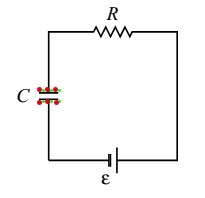
\includegraphics[width=0.33\textwidth]{images/Circuito_RC_2.png}
    }
    \subfloat[Proceso de carga.]{
        \label{fig::circuito_rc3_2}
        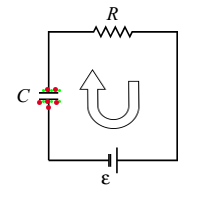
\includegraphics[width=0.33\textwidth]{images/Circuito_RC_3.png}
    }
    \subfloat[Carga completa]{
        \label{fig::circuito_rc4_2}
        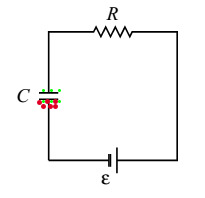
\includegraphics[width=0.33\textwidth]{images/Circuito_RC_4.png}
    }
    \caption{Fases del estado de carga de un condensador. Los puntos rojos hacen referencia a los electrones en movimiento, los puntos verdes a las cargas positivas. La flecha indica el sentido del movimiento de los electrones.}
    \label{fig::carga_condensador_2}
\end{figure}


\subsubsection{Carga del condensador}
\label{part::carga_condensador_1}
Partimos de la ecuación planteada a la hora de hacer el balance energético (\ref{eqq::balance_energetico_rc_1}). Utilizando las definiciones de capacidad del condensador y la \textit{ley de Ohm}; y posteriormente, la definición de \textit{intensidad de corriente}, derivamos a la siguiente expresión:

$$\varepsilon = \frac{q(t)}{C} + R\cdot I(t) = \frac{q(t)}{C} + R \frac{d q(t)}{d t}$$

Para resolver esta ecuación diferencial de primer orden, utilizaremos el método de separación de variables, así que la reescribimos de la siguiente forma:

$$\frac{d q(t)}{C\varepsilon - q(t)} = \frac{d t}{RC}$$

Partiendo de las condiciones iniciales, donde la carga del condensador es cero 
$$q(0) = 0$$, integramos entonces en ambos lados bajo estas condiciones

$$\int_{0}^{q(t)} \frac{d q(t)}{C\varepsilon - q(t)}  =  \int_{0}^{t} \frac{d t}{RC} $$


$$ -\ln{\left( C\varepsilon - q(t)\right)} + \ln C\varepsilon = t/{RC}$$

Despejamos $q(t)$:
{\large
$$ e^{-\ln{\left( C\varepsilon - q(t)\right)} + \ln{\left( C\varepsilon \right)}} = e^{\frac{t}{RC}}$$ }

$$\frac{1}{C\varepsilon - q(t)}C\varepsilon = e^{\frac{t}{RC}}$$

$$e^{\frac{-t}{RC}} C  \varepsilon = C\varepsilon - q(t)$$

Obteniendo finalmente

\begin{equation}
    q(t) = C\varepsilon \left( 1 - e^{\frac{-t}{RC}} \right)
    \label{eqq:q(t)_carga_rc}
\end{equation}

Además, es posible hallar que la carga máxima del condensador vendrá determinada por 

$$q_{max} = \lim_{t \to \infty} q(t) = C \cdot \varepsilon$$

\subsubsection{Intensidad de corriente}
\label{part::carga_condensador_2}
Utilizando entonces la definición de \textit{intensidad de corriente}
$$I(t) = \frac{d q(t)}{ d t}$$, si derivamos la expresión de carga del condensador obtenemos que

\begin{equation}
    I(t) = \frac{\varepsilon}{R} e^{\frac{-t}{RC}}
\end{equation}

\subsubsection{Diferencia de potencial resistencia (R)}
\label{part::carga_condensador_3}
Para obtener la diferencia de potencial entre los bornes de la resistencia, hacemos uso de la \textit{ley de Ohm}

\begin{equation}
    V_R(t) = R \cdot I(t)
    \label{eqq::dif_potencial_resistencia}
\end{equation}


, que usando la expresión resultante en \ref{part::carga_condensador_2} obtenemos

\begin{equation}
    V_R(t) = R \cdot e^{\frac{-t}{RC}}
\end{equation}

\subsubsection{Diferencia de potencial en el condensador (C)}
\label{part::carga_condensador_4}
Por otro lado, la diferencia de potencial entre los terminales del condensador hacemos uso de la definición de capacidad del mismo 

\begin{equation}
    V_C(t) = \frac{q(t)}{C}
    \label{eqq::dif_potencial_condensador}
\end{equation}

, así que usando la expresión obtenida en \ref{part::carga_condensador_1} obtenemos

\begin{equation}
    V_C(t) = \varepsilon \left( 1- e^{\frac{-t}{RC}}\right)
\end{equation}



\subsection{Circuito RC en descarga}
\begin{figure}[!h]
    \centering
    \subfloat[$t=0$. Carga previa.]{
        \label{fig::circuito_rc5_2}
        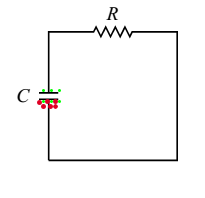
\includegraphics[width=0.33\textwidth]{images/Circuito_RC_5.png}
    }
    \subfloat[Proceso de descarga]{
        \label{fig::circuito_rc6_2}
        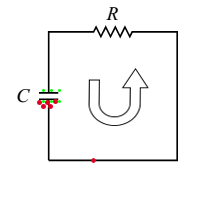
\includegraphics[width=0.33\textwidth]{images/Circuito_RC_6.png}
    }
    \subfloat[Condensador con $q=0$]{
        \label{fig::circuito_rc7_2}
        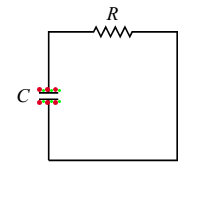
\includegraphics[width=0.33\textwidth]{images/Circuito_RC_7.png}
    }
    \caption{Descarga de un condensador.}
    \label{fig::descarga_condensador_2}
\end{figure}


\subsubsection{Carga del condensador}

\label{part::descarga_condensador_1}
Partimos de la ecuación planteada a la hora de hacer el balance energético (\ref{eqq::balance_energetico_rc_2}). Utilizando las definiciones de capacidad de condensador y la \textit{ley de Ohm}; y posteriormente, la definición de \textit{intensidad de corriente}, obtenemos que:

$$0 = \frac{q(t)}{C} + R\frac{d q(t)}{d t}$$

Para resolver esta ecuación diferencial, utilizaremos el método de separación de variables, así que la reescribimos de la siguiente manera:

$$\frac{-d t}{RC} = \frac{d q(t)}{q(t)}$$

Si partimos de un condensador completamente cargado, donde la carga en el instante inicial se corresponde a 

$$q(0) = q_{max} = C \cdot \varepsilon$$,

integramos entonces en ambos lados,

$$\int_{C\varepsilon}^{q(t)} \frac{d q(t)}{q(t)}  = \int_{0}^{t} \frac{-d t}{RC} $$

Resolvemos en ambos lados:


$$\ln{q(t)} - \ln{C\varepsilon} = \frac{-t}{RC}$$

{\large
$$ e^{\ln{q(t)} - \ln{C\varepsilon}} = e^{\frac{-t}{RC}}$$ }

$$q(t)\frac{1}{C\varepsilon} = e^{\frac{-t}{RC}} $$

Despejamos $q(t)$:

\begin{equation}
    q(t) = C \varepsilon e^{\frac{-t}{RC}}
    \label{eqq::q(t)_descarga_rc}
\end{equation}


\subsubsection{Intensidad de corriente}
\label{part::descarga_condensador_2}
Utilizando la definición de \textit{intensidad de corriente}

$$I(t) = \frac{d q(t)}{d t}$$

y la expresión correspondiente a la carga del condensador en estado de dispación de energía (\ref{eqq::q(t)_descarga_rc}), obtenemos:

\begin{equation}
    I(t) = -\frac{\varepsilon}{R} e^{\frac{-t}{RC}} 
\end{equation}



\subsubsection{Diferencia de potencial en la resistencia}
\label{part::descarga_condensador_3}
Para obtener la diferencia de potencial entre los bornes de la resistencia, usamos la \textit{ley de Ohm}

$$V_R(t) = R \cdot I(t)$$
, que usando la expresión resultante en \ref{part::descarga_condensador_2} obtenemos:

\begin{equation}
    V_R(t) = -\varepsilon \cdot e^{\frac{-t}{RC}}
\end{equation}


\subsubsection{Diferencia de potencial en el condensador}
\label{part::descarga_condensador_4}
Para calcular la diferencia de potencial en los terminales del condensador, usamos la definición de capacidad en un conductor
$$V_C(t) = \frac{q(t)}{C}$$
, así que usando la expresión obtenida en \ref{part::descarga_condensador_1} obtenemos:

\begin{equation}
    V_C(t) = \varepsilon  e^{\frac{-t}{RC}}
\end{equation}



\subsection{Energía del campo eléctrico}
\label{part::energia_condensador}
Si partimos de un condensador completamente descargado, entonces la energía en ese momento también es cero.

$$E(0) = 0$$

Por definición, sabemos que la carga en el condensador es

$$q(t) = C \cdot V_C(t)$$, 

y que la intensidad de corriente que lo atraviesa viene dada entonces por la siguiente expresión

$$I(t) = C \frac{d V_C(t)}{d t}$$

Usando las definiciones de energía y potencia consumidas por el condensador

$$d E(t) = p(t)  d t = V_C(t) I(t) d t $$

obtenemos que la energía almacenada en es la solución de la siguiente ecuación diferencial de primer orden:

$$d E(t) = C \cdot V_C(t) d V_C(t)$$

Resolvemos integrando usando las condiciones iniciales previas

$$\int_{0}^{E(t)} d E(t) = C \int_{0}^{V_C(t)} V_C(t) d V_C(t) $$

$$E(t) = C \left[ \frac{V_C(t)^2}{2} \right]_{0}^{V_C(t)}$$

Luego, la energía almacenada en el condensador viene dada por:

\begin{equation}
    E(t) = \frac{1}{2}CV_C(t)^2
\end{equation}

, dónde $V_C(t)$ es la diferencia de potencial en el condensador.


\end{document}